\section{Gradient Computation}
I managed to successfully write the functions to correctly compute the gradient analytically.
I tested my implementation by computing the gradients using ComputeGradsNumSlow.m.
Then I compared my results with the numerical approaches by calculating the absolute difference of each gradient element as in equations below.
Then I checked those against a threshold (1e-5). 
When using the reduced set with \texttt{n=2} on a 3 layer network with [50, 50] nodes in the hidden layers and using ComputeGradsNumSlow.m 
I get a maximum error of 
\begin{itemize}
    \item \texttt{diff\_W1\_max = 2.2204e-11}
    \item \texttt{diff\_b1\_max = 2.2204e-11}
    \item \texttt{diff\_gamma1\_max = 2.2356e-11}
    \item \texttt{diff\_beta1\_max = 2.2356e-11}
    \item \texttt{diff\_W2\_max = 4.1234e-13}
    \item \texttt{diff\_b2\_max = 2.2204e-16}
    \item \texttt{diff\_gamma2\_max = 3.3339e-11}
    \item \texttt{diff\_beta2\_max = 3.3339e-11}
    \item \texttt{diff\_W3\_max = 2.3122e-11}
    \item \texttt{diff\_b3\_max = 2.4201e-11}

\end{itemize}
These errors are small enough to conclude that my implementation works. \\ 
\begin{equation}\label{eq:diffw}
    diff\_W = abs(ngrad\_W - grad\_W)
\end{equation}
\begin{equation}\label{eq:diffb}
    diff\_b = abs(ngrad\_b - grad\_b)
\end{equation}
\begin{equation}\label{eq:diffgamma}
    diff\_gamma = abs(ngrad\_gamma - grad\_gamma)
\end{equation}
\begin{equation}\label{eq:diffbeta}
    diff\_beta = abs(ngrad\_beta - grad\_beta)
\end{equation}

\clearpage
\section{3-layer Network}
Training a 3-layer network with [50, 50] hidden nodes, lambda=0.005, eta\_min=1e-5, eta\_max=1e-1, cycles=2, n\_batch=100, n\_s=5*45000/n\_batch.
\subsection{Without batch normalization}
accuracy\_validation = 54.1\%\\
accuracy\_test = 53.05\%
\begin{figure}[ht]
    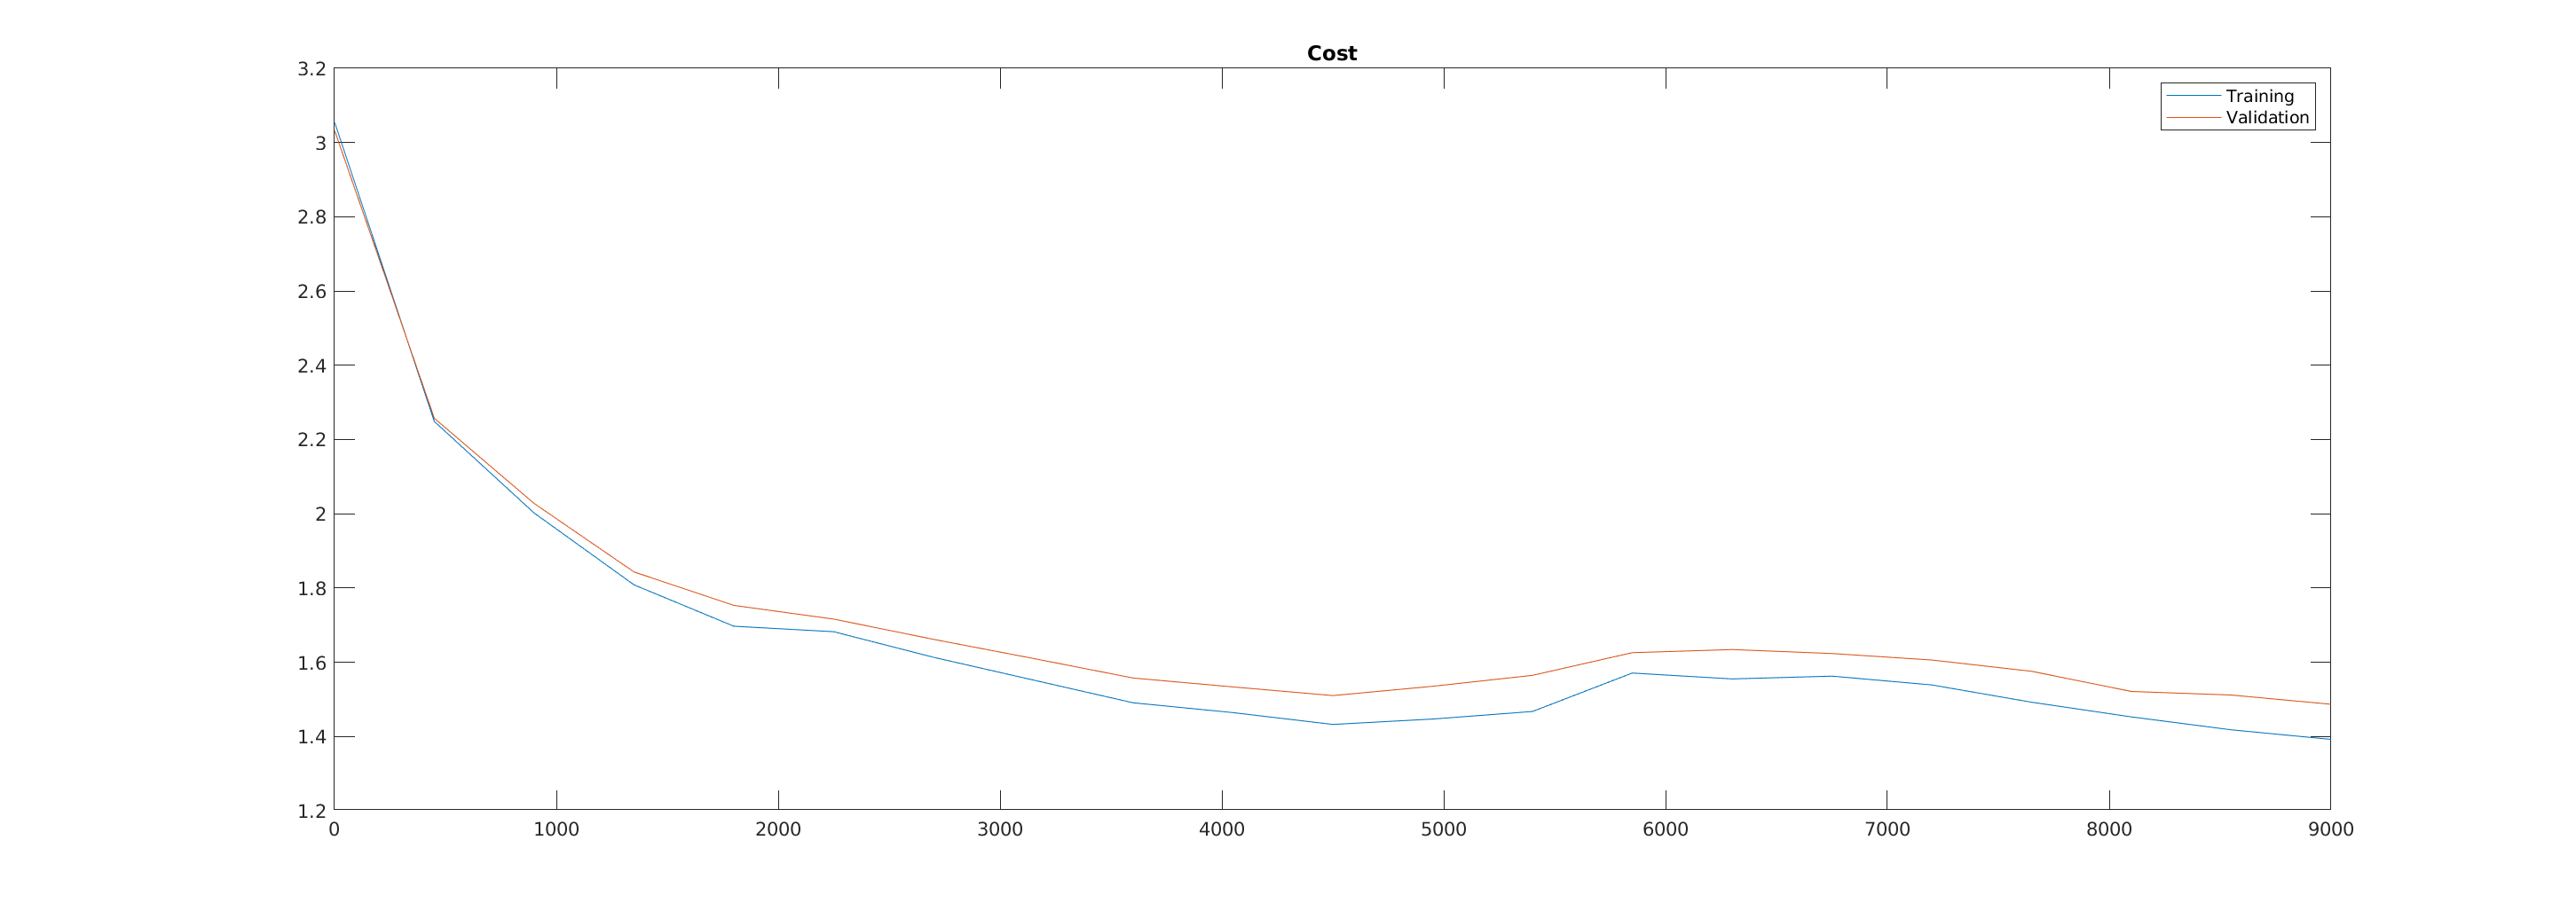
\includegraphics[width=\textwidth]{../code/result_pics/cost_lambda=0.00500_ns=2250_cycles=2_k=3_bn=0.png}
    \caption{Loss, 3-layer without batch normalization}
\end{figure}

\subsection{With batch normalization}
accuracy\_validation = 55.1\%\\
accuracy\_test = 53.95\%
\begin{figure}[ht]
    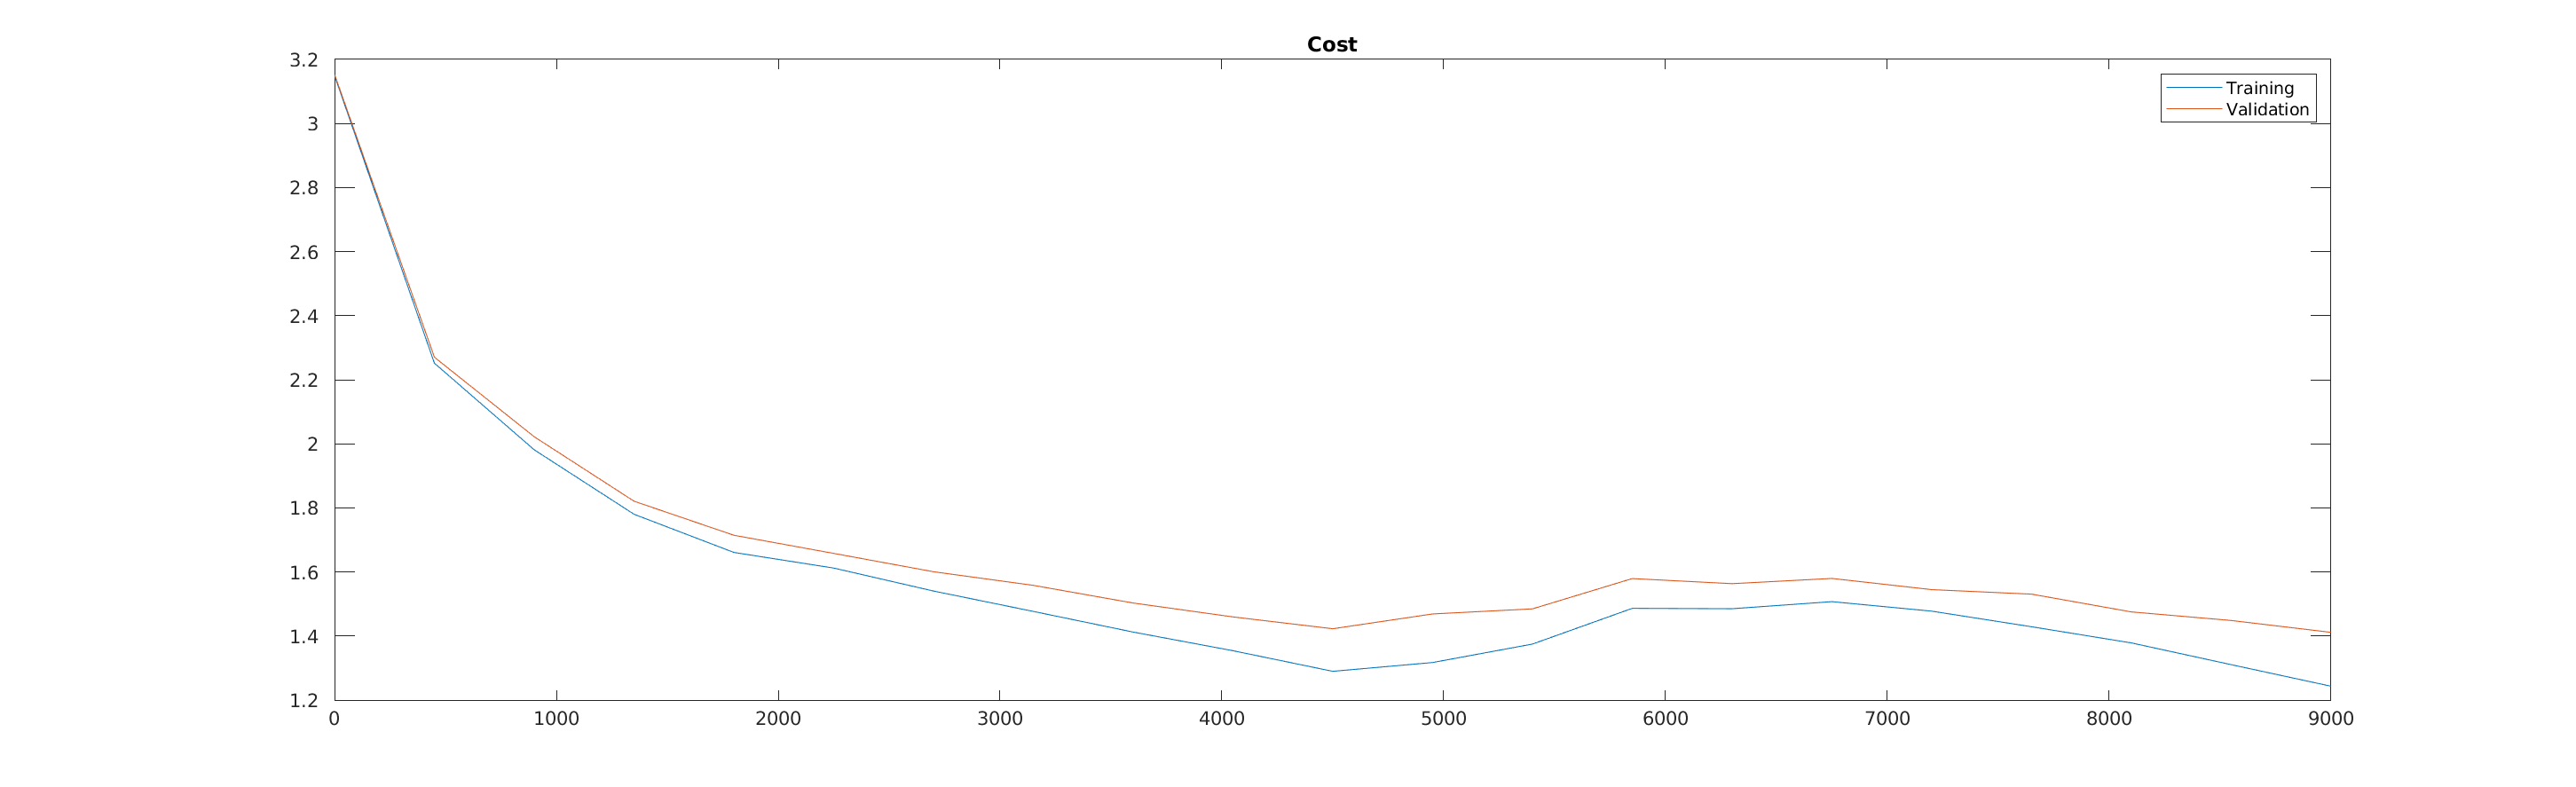
\includegraphics[width=\textwidth]{../code/result_pics/cost_lambda=0.00500_ns=2250_cycles=2_k=3_bn=1.png}
    \caption{Loss, 3-layer with batch normalization}
\end{figure}
\clearpage

\section{9-layer Network}
Training a 9-layer network with [50; 30; 20; 20; 10; 10; 10; 10] hidden nodes, lambda=0.005, eta\_min=1e-5, eta\_max=1e-1, cycles=2, n\_batch=100, n\_s=5*45000/n\_batch.
\subsection{Without batch normalization}
accuracy\_validation = 47.1\%\\
accuracy\_test = 45.18\%
\begin{figure}[ht]
    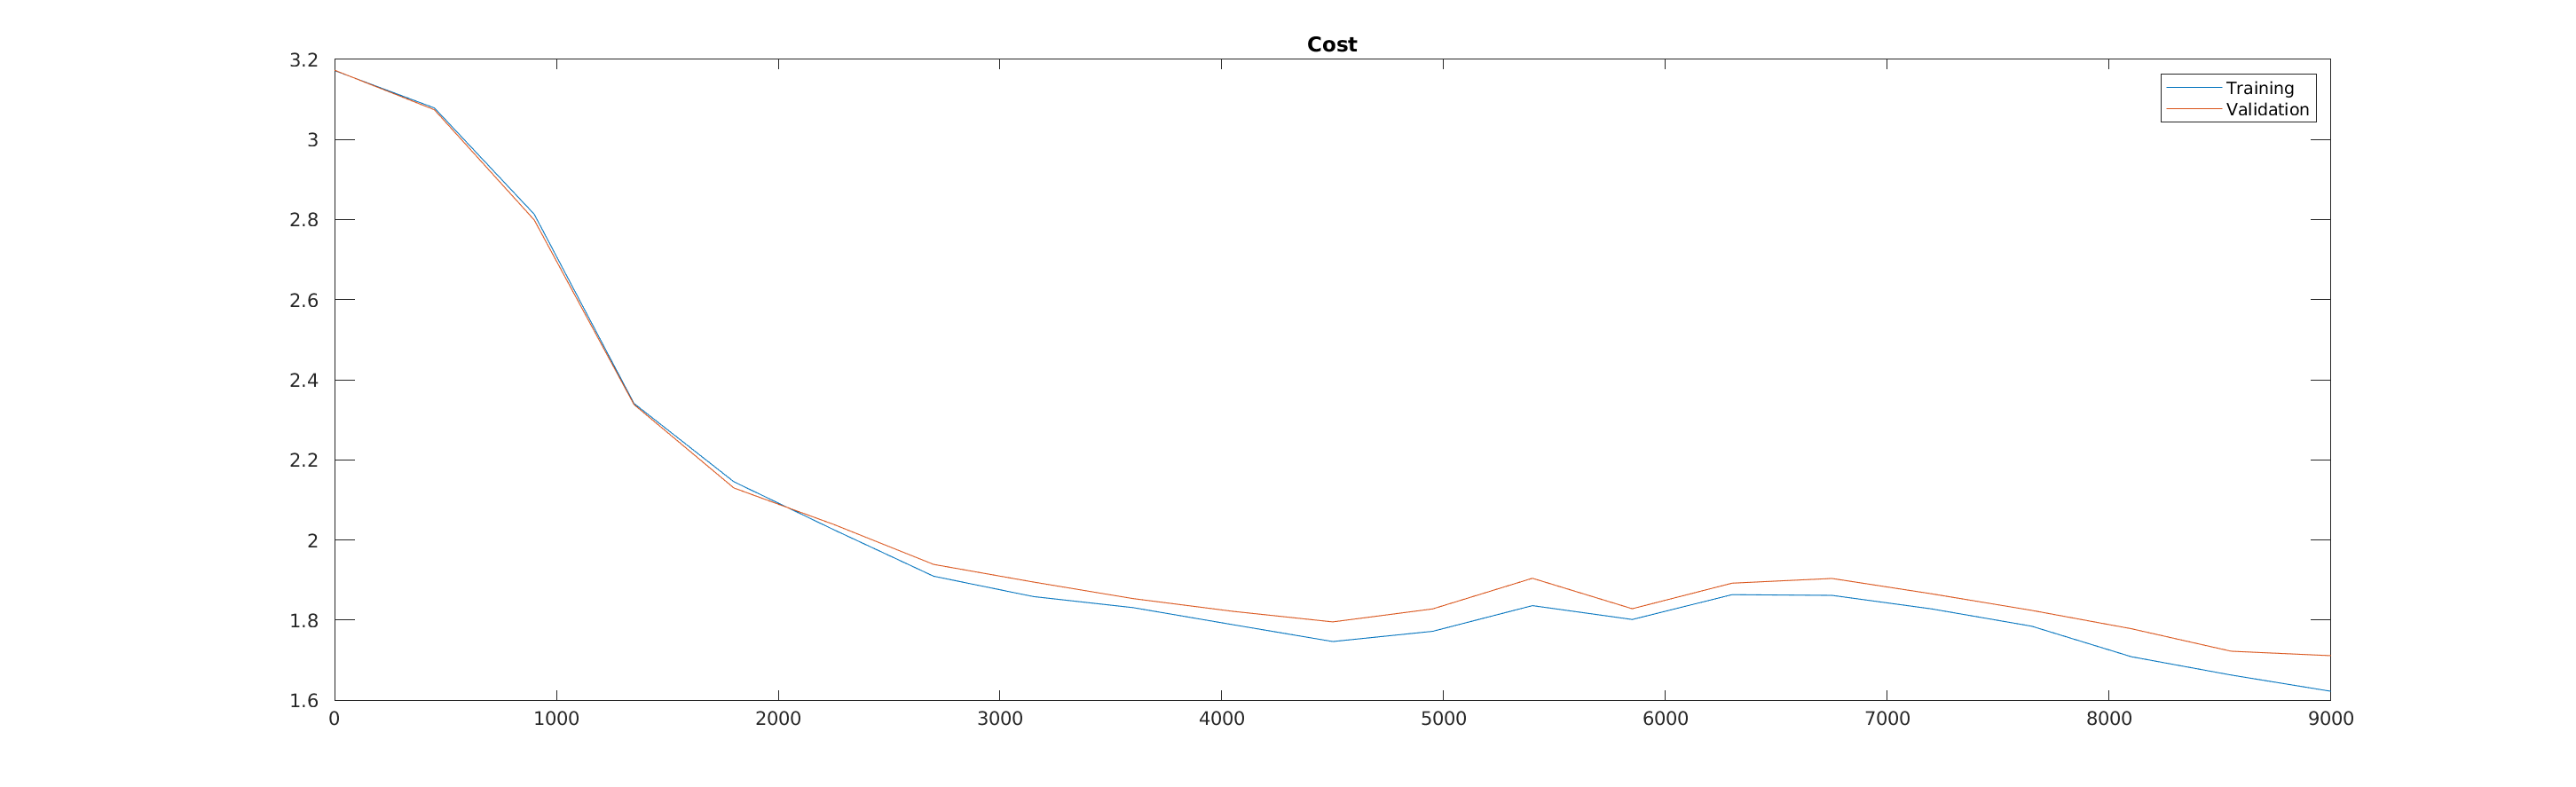
\includegraphics[width=\textwidth]{../code/result_pics/cost_lambda=0.00500_ns=2250_cycles=2_k=9_bn=0.png}
    \caption{Loss, 9-layer without batch normalization}
\end{figure}

\subsection{With batch normalization}
accuracy\_validation = 52.3\%\\
accuracy\_test = 51.6\%
\begin{figure}[ht]
    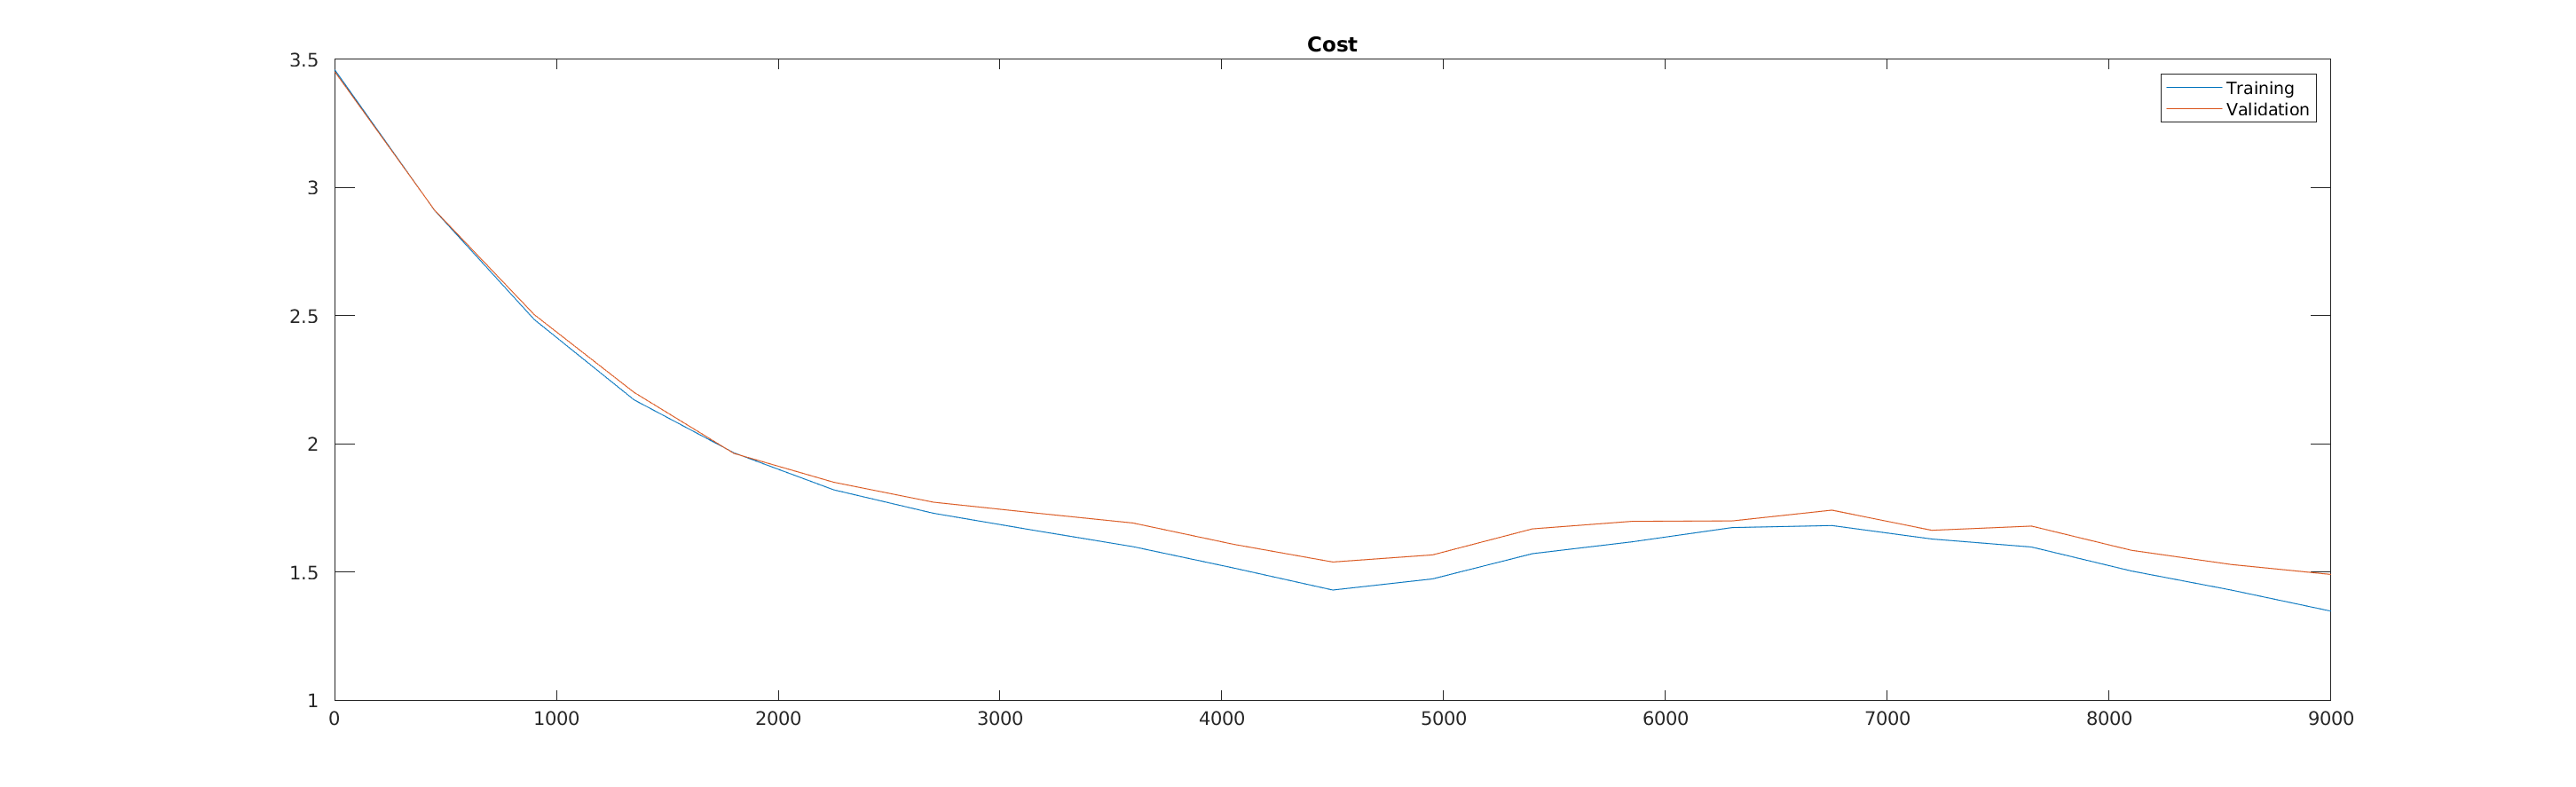
\includegraphics[width=\textwidth]{../code/result_pics/cost_lambda=0.00500_ns=2250_cycles=2_k=9_bn=1.png}
    \caption{Loss, 9-layer with batch normalization}
\end{figure}
\clearpage

\section{Optimizing 3-layer network}
To optimize I first performed a coarse lambda search over a uniform grid between \texttt{lambda=1e-5} and \texttt{lambda=1e-1}.
I sampled 20 lambdas in the interval and trained for 2 cycles.
This resulted in a best result (based on validation accuracy) at \texttt{lambda=0.00527} and \texttt{accuracy=55.5\%}. 
Then I performed a finer, random search between \texttt{lambda=0.00001} and \texttt{lambda=0.01}.
I sampled 20 lambdas randomly and trained for 2 cycles.
This resulted in a best result (based on validation accuracy) at \texttt{lambda=0.00564} and \texttt{accuracy=55.6\%}.
Then I trained the network with this lambda for 3 cycles, which resulted in a test accuracy of 54.27\% and
a validation accuracy of 56.1\%.
\begin{figure}[ht]
    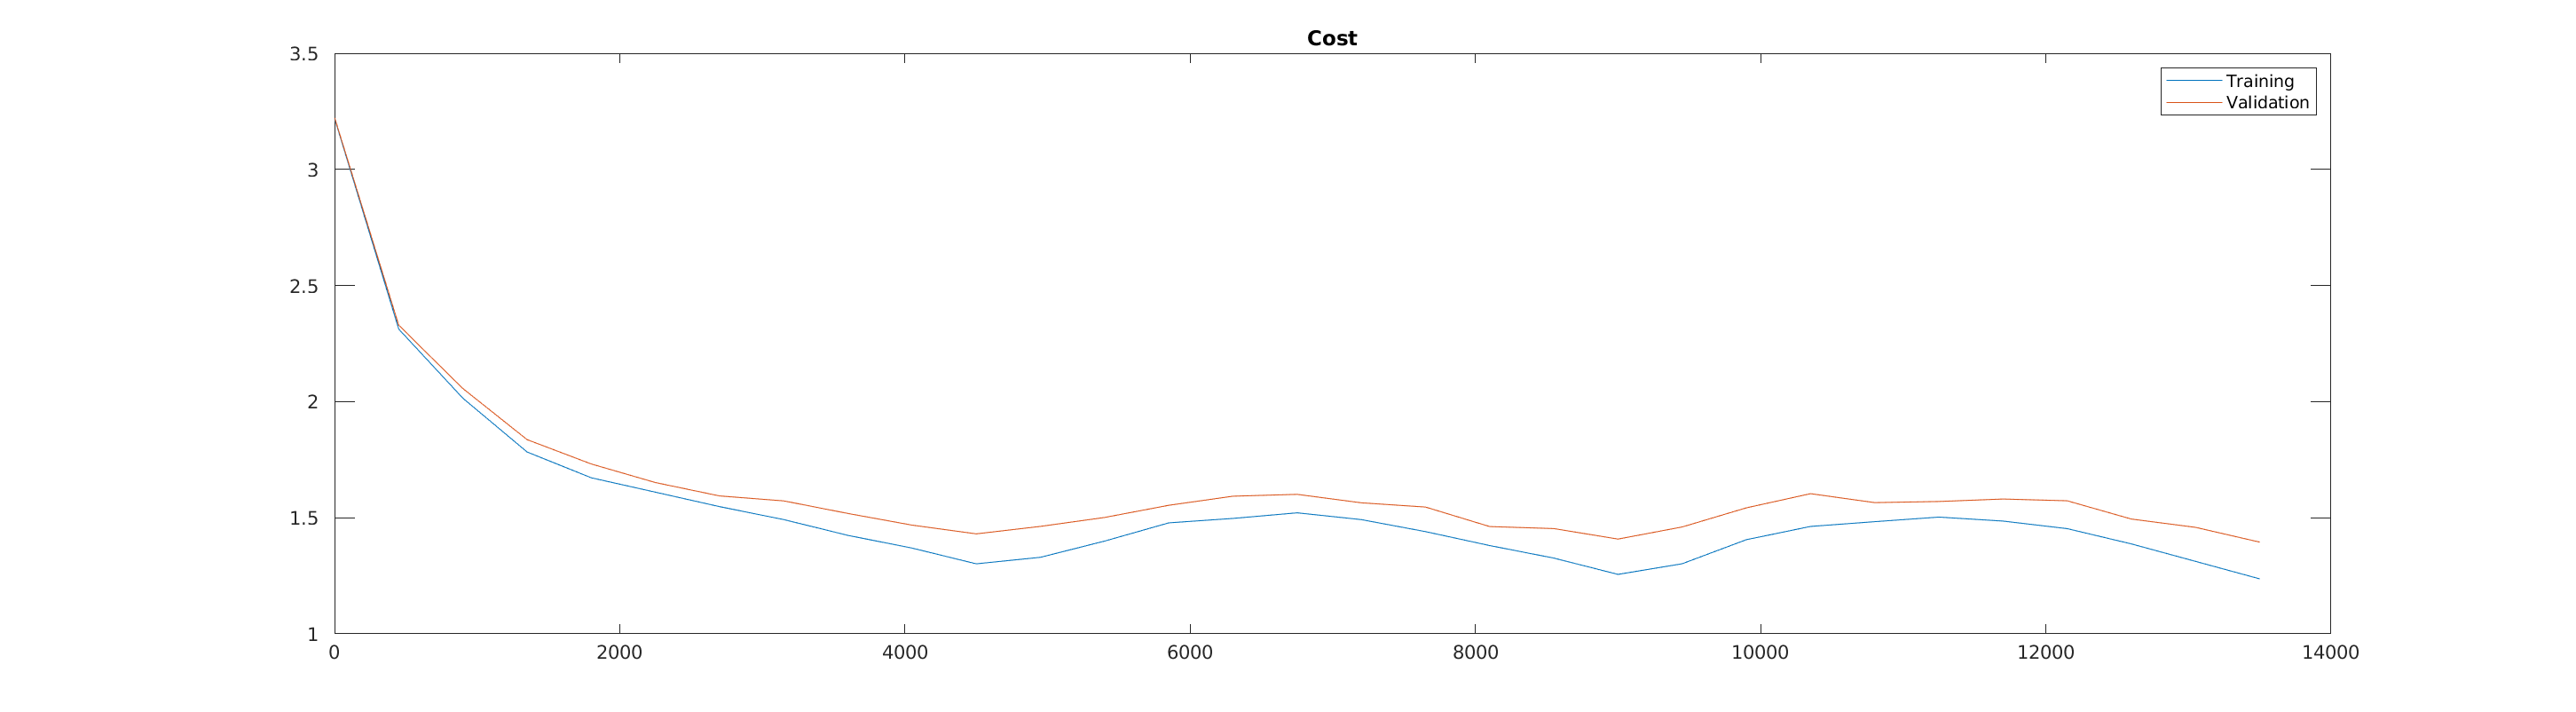
\includegraphics[width=\textwidth]{../code/result_pics/cost_lambda=0.00564_ns=2250_cycles=3_k=3_bn=1.png}
    \caption{Loss, optimized 3-layer with batch normalization}
\end{figure}
\begin{figure}[ht]
    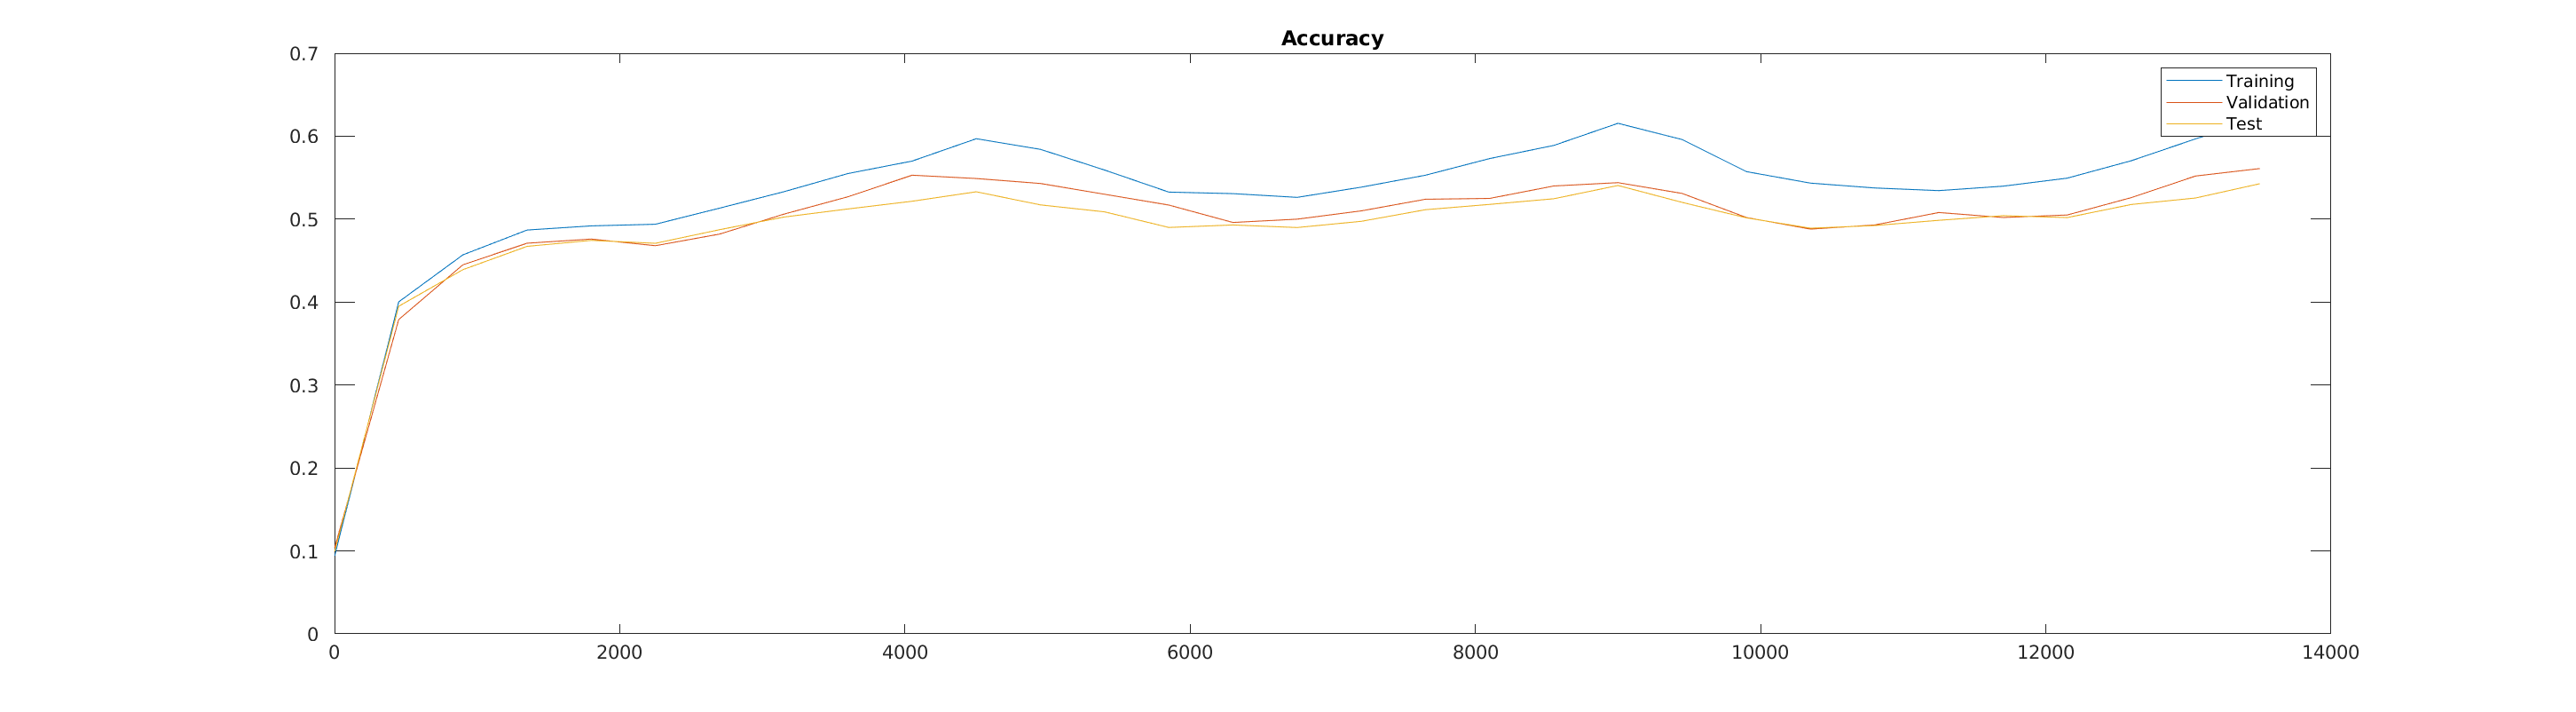
\includegraphics[width=\textwidth]{../code/result_pics/accuracy_lambda=0.00564_ns=2250_cycles=3_k=3_bn=1.png}
    \caption{Accuracy, optimized 3-layer with batch normalization}
\end{figure}
\clearpage

\section{Sensitivity to initialization}
Instead of He initialization initialize the weights of the network with a normal distribution with the same sigma on each layer.
Test this for 3 different sigmas.
\subsection{sig=1e-1}
\subsubsection{Without batch normalization}
accuracy\_validation = 53.2\%\\
accuracy\_test = 53.24\%
\begin{figure}[ht]
    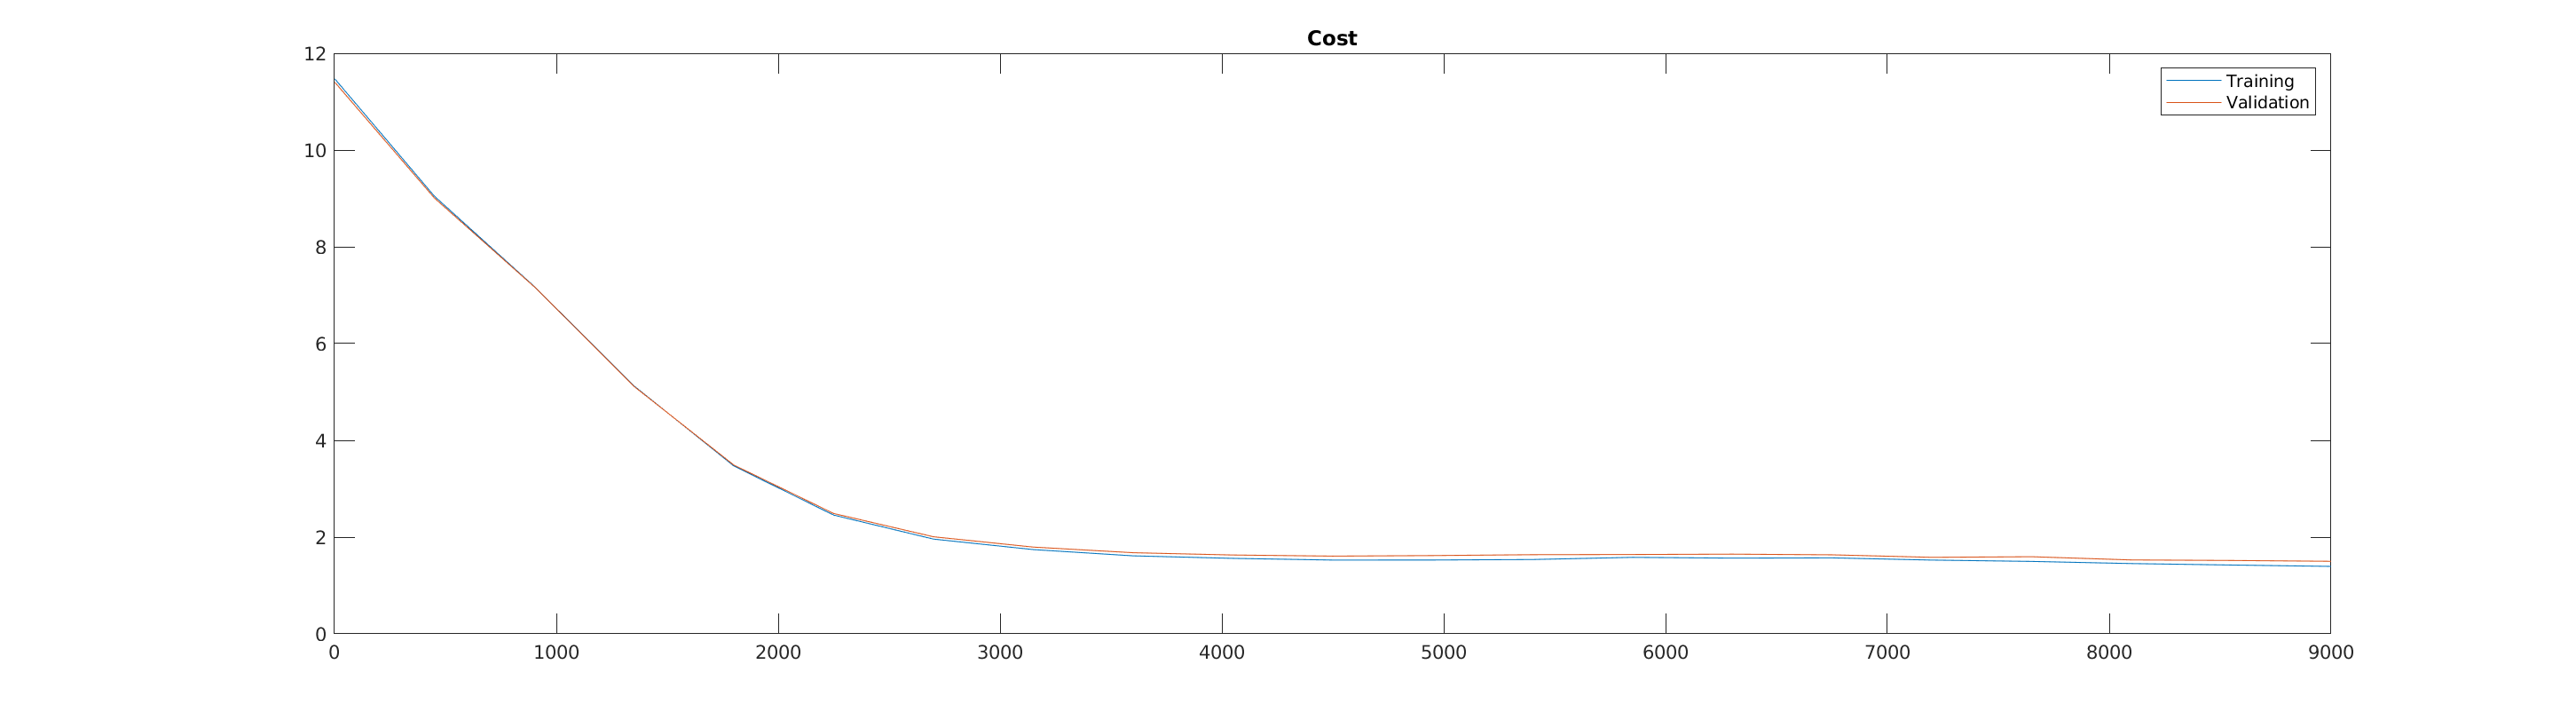
\includegraphics[width=\textwidth]{../code/result_pics/cost_lambda=0.00500_ns=2250_cycles=2_k=3_sig=0.10000_bn=0.png}
    \caption{Loss, sig=1e-1, 3-layer without batch normalization}
\end{figure}

\subsubsection{With batch normalization}
accuracy\_validation = 53.7\%\\
accuracy\_test = 53.49\%
\begin{figure}[ht]
    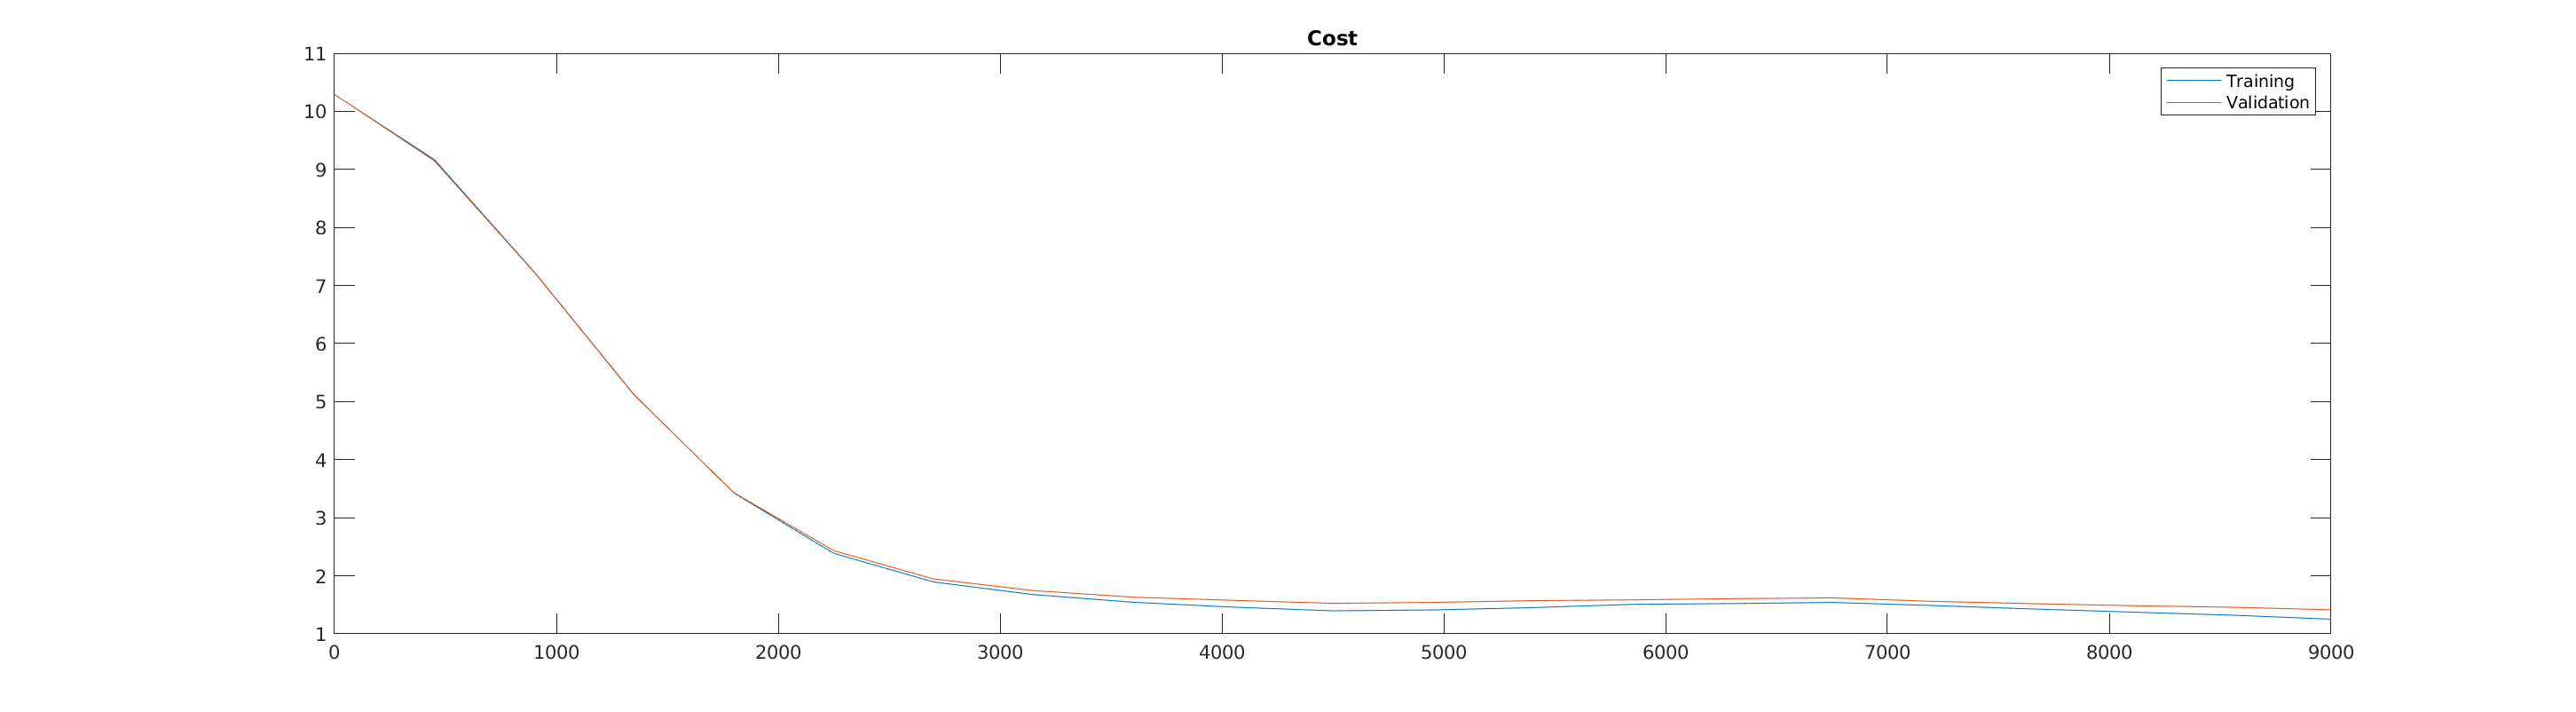
\includegraphics[width=\textwidth]{../code/result_pics/cost_lambda=0.00500_ns=2250_cycles=2_k=3_sig=0.10000_bn=1.png}
    \caption{Loss, sig=1e-1, 3-layer with batch normalization}
\end{figure}

\clearpage

\subsection{sig=1e-3}
\subsubsection{Without batch normalization}
accuracy\_validation = 50.6\%\\
accuracy\_test = 50.29\%
\begin{figure}[ht]
    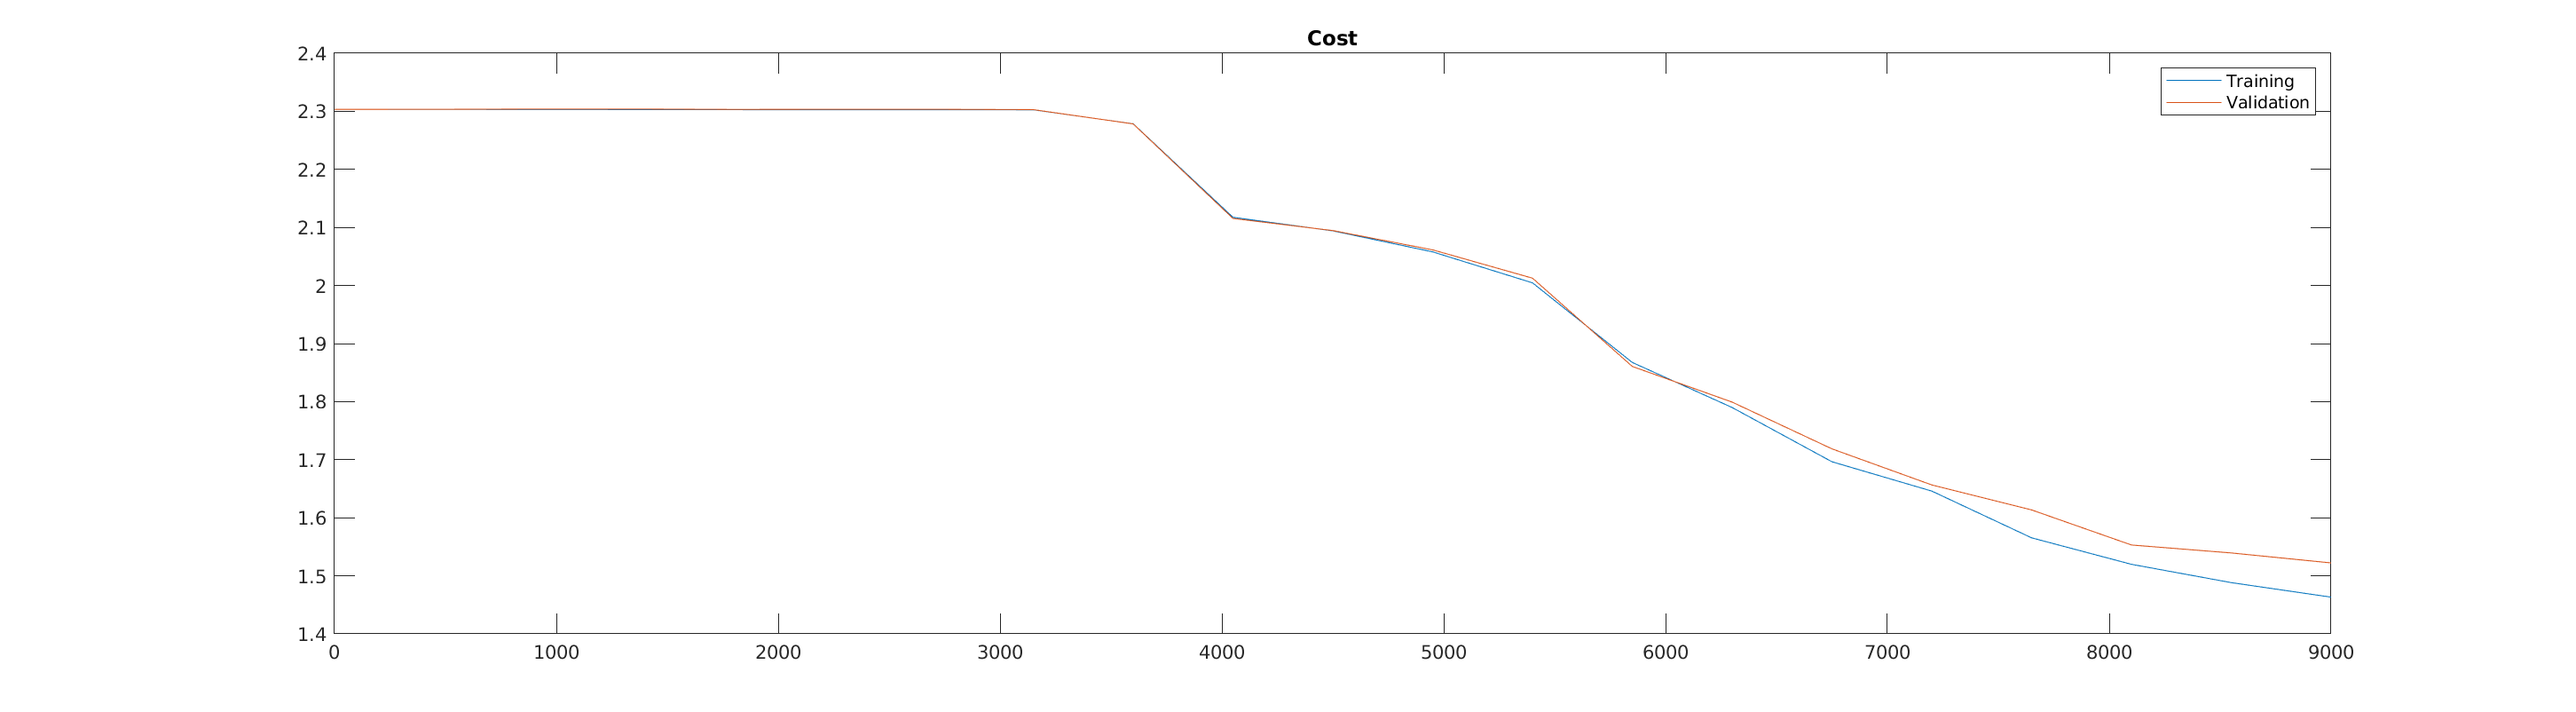
\includegraphics[width=\textwidth]{../code/result_pics/cost_lambda=0.00500_ns=2250_cycles=2_k=3_sig=0.00100_bn=0.png}
    \caption{Loss, sig=1e-3, 3-layer without batch normalization}
\end{figure}

\subsubsection{With batch normalization}
accuracy\_validation = 54.9\%\\
accuracy\_test = 53.88\%
\begin{figure}[ht]
    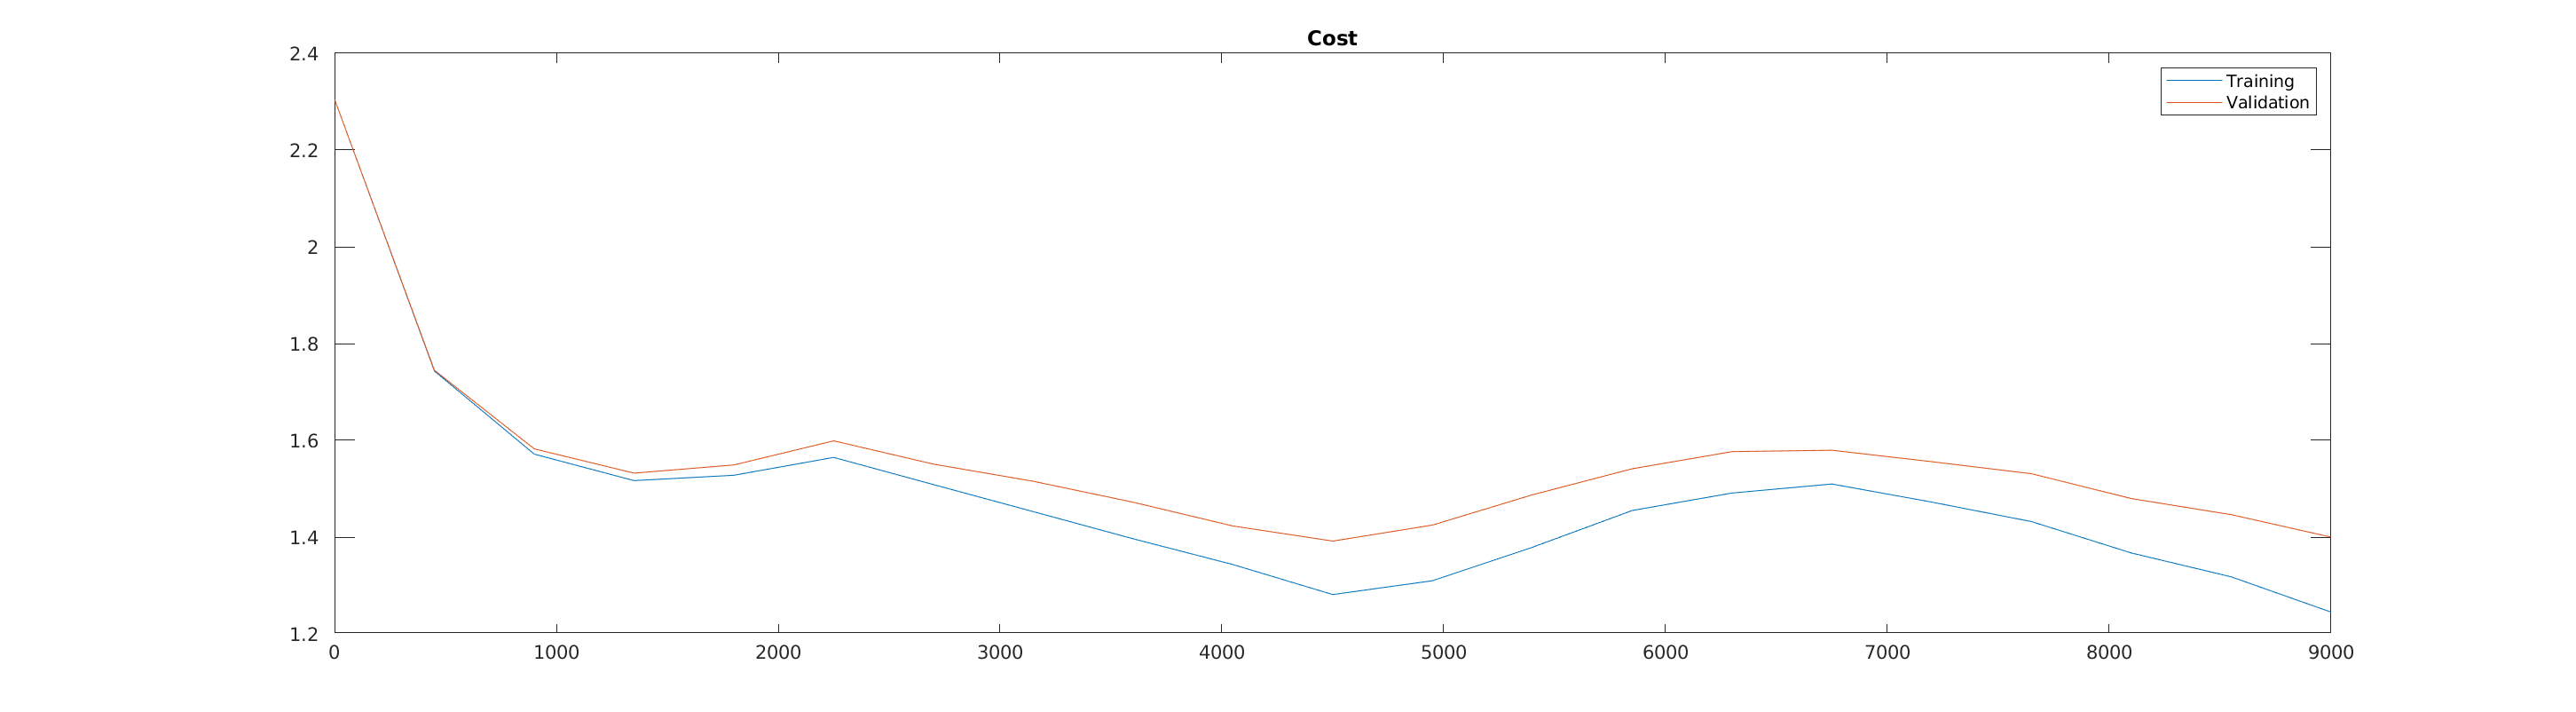
\includegraphics[width=\textwidth]{../code/result_pics/cost_lambda=0.00500_ns=2250_cycles=2_k=3_sig=0.00100_bn=1.png}
    \caption{Loss, sig=1e-3, 3-layer with batch normalization}
\end{figure}
\clearpage

\subsection{sig=1e-4}
\subsubsection{Without batch normalization}
accuracy\_validation = 7.8\%\\
accuracy\_test = 10\%
\begin{figure}[ht]
    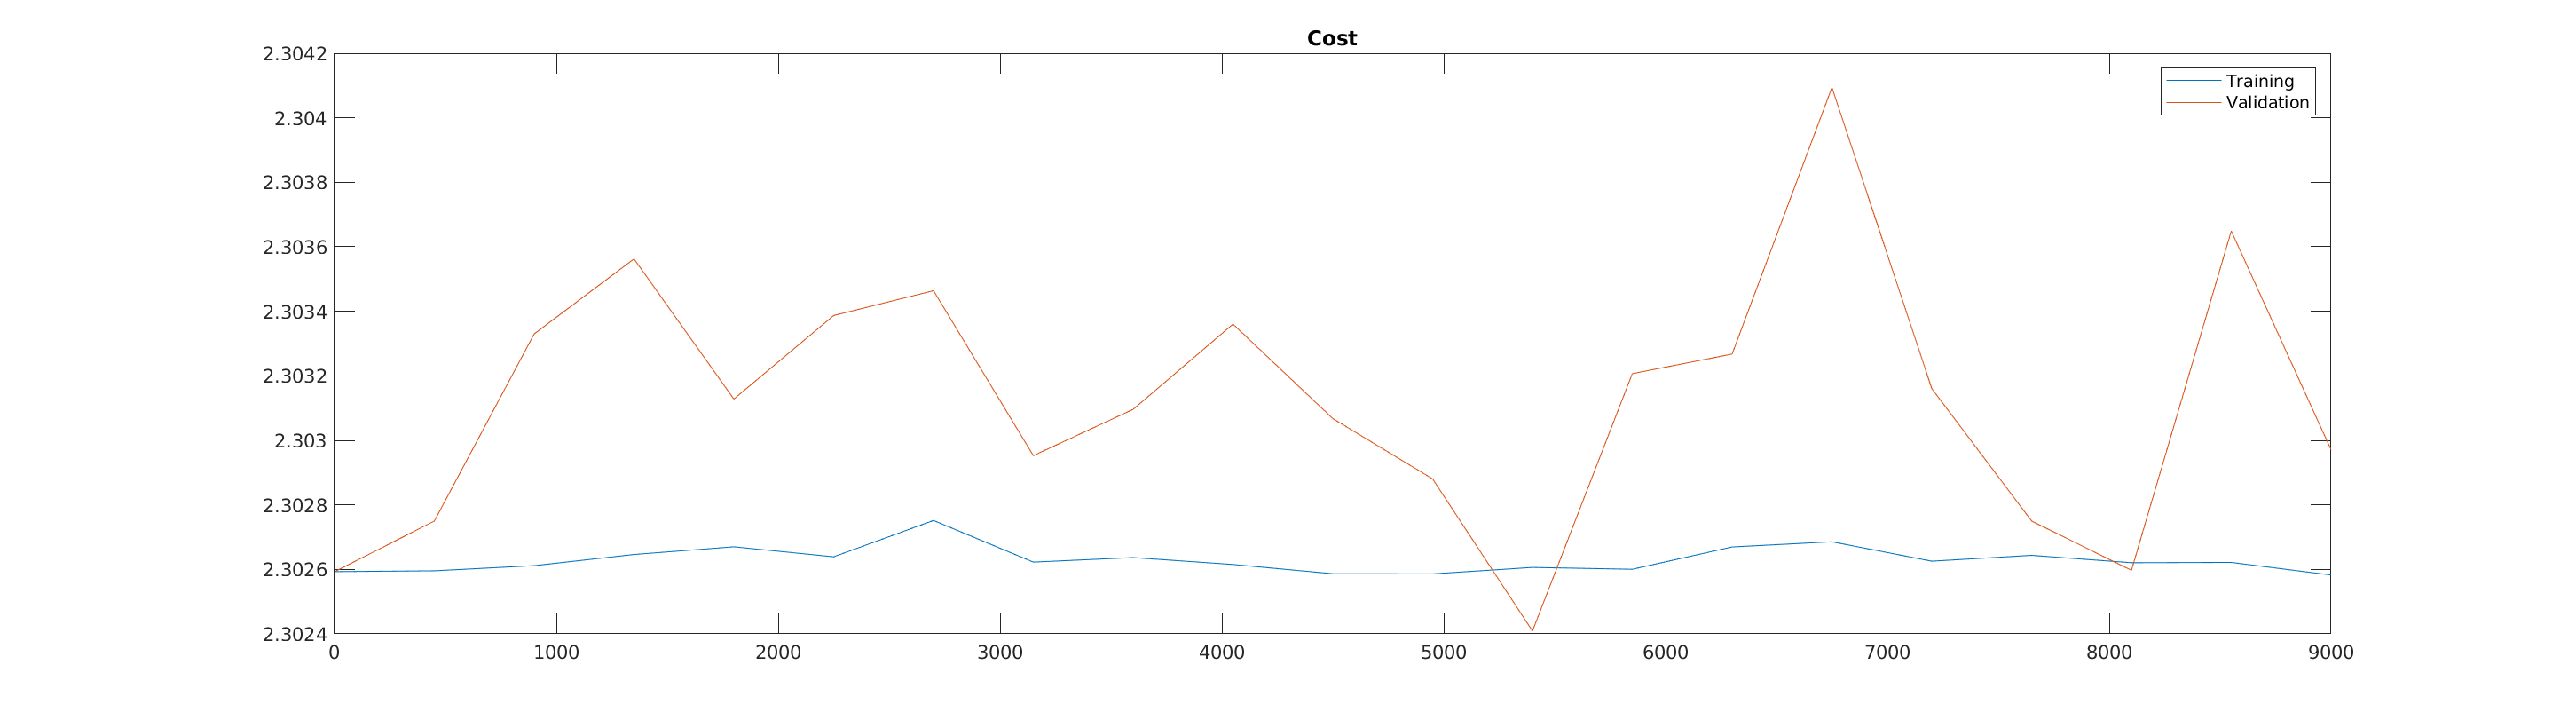
\includegraphics[width=\textwidth]{../code/result_pics/cost_lambda=0.00500_ns=2250_cycles=2_k=3_sig=0.00010_bn=0.png}
    \caption{Loss, sig=1e-4, 3-layer without batch normalization}
\end{figure}

\subsubsection{With batch normalization}
accuracy\_validation = 55.2\%\\
accuracy\_test = 53.44\%
\begin{figure}[ht]
    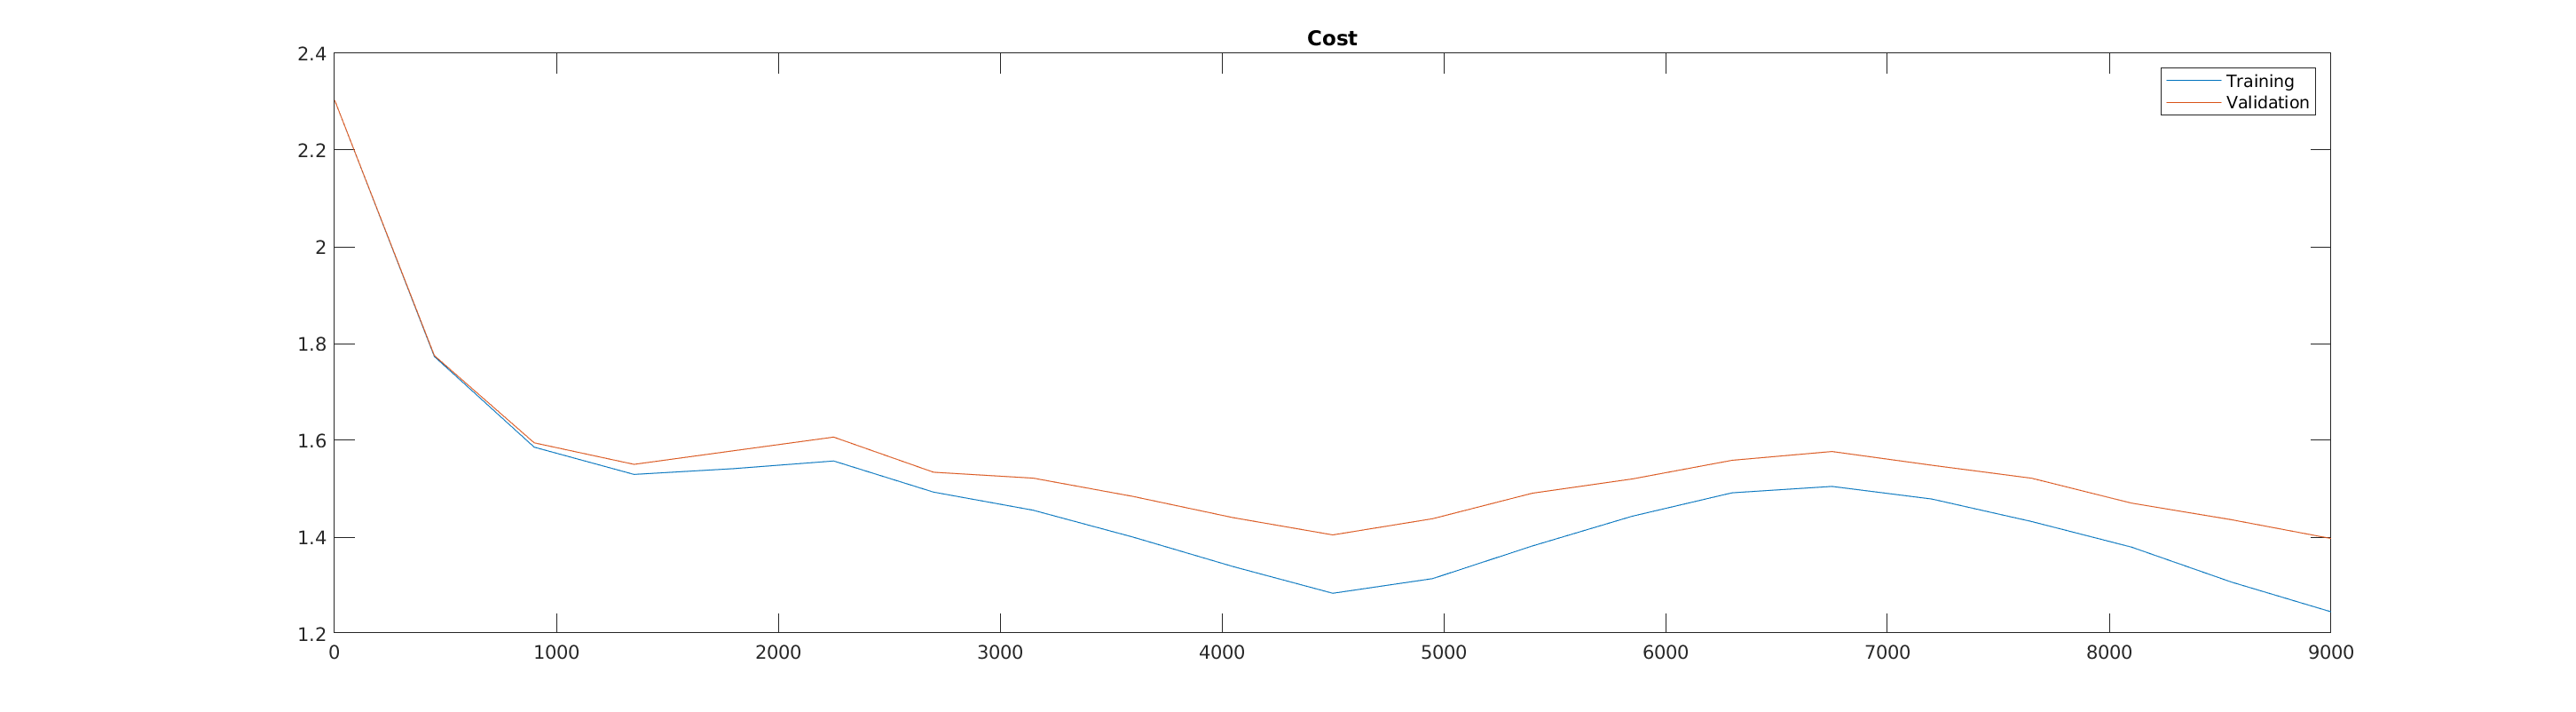
\includegraphics[width=\textwidth]{../code/result_pics/cost_lambda=0.00500_ns=2250_cycles=2_k=3_sig=0.00010_bn=1.png}
    \caption{Loss, sig=1e-4, 3-layer with batch normalization}
\end{figure}
\clearpage
\subsection{Conclusion}
From the experiment we can see that batch normalization makes the training much more stable. The effect is best visible in the 
experiment with sig=1e-4. The initialization is very bad for training and without batch normalization the network achieves a
very low test accuracy of only 10\%. If we use batch normalization we achieve 53.44\%, which is (almost) the same test accuracy as the optimized network which 
used a good initialization (Xavier).




